\en{Let $O$ be the centre of the circumcircle of an acute triangle $ABC$. The line $AC$ intersects the circumcircle of the triangle $ABO$ a second time at $S$. Prove that the line $OS$ is perpendicular to the line $BC$.

\textbf{Solution 1:}
Reformulation of the conclusion: To prove that $OS$ is perpendicular to $BC$, we introduce $T$ to be the intersection of $OS$ with $BC$ and prove that $\angle CTS=90^\circ$. Thanks to angle chasing, we observe the following.

\begin{enumerate}
    \item Since $AOBS$ are on a circle, we have $\angle ASO=\angle ABO$.
    \item Since $O$ is the centre of the circle $ABC$, it holds $OA=OB$ and therefore the triangle $AOB$ is isosceles at $O$. Hence $\angle AOB=180^\circ -2\cdot\angle ABO$.
    \item Since $O$ is the centre of the circle $ABC$, it holds $\angle ACB=\frac{1}{2}\cdot\angle AOB$.
\end{enumerate}

Combining the observations above, we get
\[
\angle SCT=\angle ACB\stackrel{\text{(c)}}{=}\frac{1}{2}\angle AOB\stackrel{\text{(b)}}{=}90^\circ -\angle ABO\stackrel{\text{(a)}}{=}90^\circ -\angle ASO=90^\circ -\angle CST.
\]
Hence, since the angles of the triangle $CTS$ sum up to $180^\circ$, we conclude
\[
\angle CTS=180^\circ-\angle SCT-\angle CST=90^\circ.
\]

\textbf{Solution 2:}
Reformulation of the conclusion: To prove that $OS$ is perpendicular to $BC$, we prove that the triangle $CSB$ is isosceles at $S$. Indeed, if the triangle $CSB$ is isosceles at $S$, then the perpendicular bisector of the segment $BC$ goes through $S$. However, the perpendicular bisector of the segment $BC$ also goes through $O$, because, $O$ being the centre of the circle $ABC$, it holds $OC=OB$. Hence, the line $OS$ is the perpendicular bisector of $BC$, and is, in particular, perpendicular to $BC$.

Thanks to angle chasing, we observe the following.

\begin{enumerate}
    \item Since $O$ is the centre of the circle $ABC$, it holds $OB=OC$ and thus $\angle OCB=\angle OBC$.
    \item Since $O$ is the centre of the circle $ABC$, it holds similarly $\angle OCA=\angle OAC$.
    \item Since $AOBS$ are on a circle, we have $\angle OBS=\angle OAC$.
\end{enumerate}

Hence, we conclude
\[
\angle SCB=\angle ACB=\angle ACO+\angle OCB\stackrel{\text{(a)\&(b)}}{=}\angle OAC+\angle OBC\stackrel{\text{(c)}}{=}\angle OBS+\angle OBC=\angle SBC.
\]

So, the triangle $CSB$ is indeed isosceles at $S$.

\begin{center}
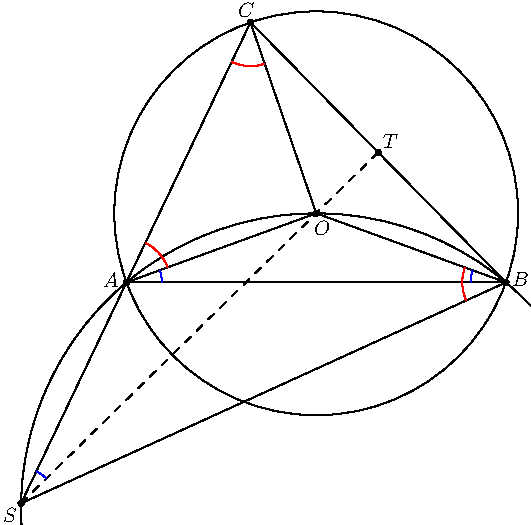
\includegraphics{g1fig.pdf}
\end{center}

\bigskip

\textbf{Marking Scheme}

\begin{itemize}
    \item 2P: reformulation of the conclusion in a statement of the kind:
    \begin{itemize}
    \item $\angle SCT=90^\circ-\angle CST$ or $\angle SCB=90^\circ-\angle CSO$
    \item $CSB$ is isosceles at $S$
    \end{itemize}
    \item 1P: any useful statement involving the cyclic quadrilateral $AOBS$ (eg.\ $\angle OBS=\angle CAO$ or $\angle ASO=\angle ABO$)
    \item $\leq$ 2P: 1P for any useful statement involving the centre $O$ of the circle $ABC$ (eg.\ $\angle ACO=\frac{1}{2}\cdot \angle AOB$, $\angle OCB=\angle OBC$, $\angle OCA=\angle OAC$, $\angle OBA=\angle OAB$) 
    \item 2P: conclude
\end{itemize}
}

\de{Sei $ABC$ ein spitzwinkliges Dreieck mit Umkreismittelpunkt $O$. Die Gerade $AC$ schneidet den Umkreis des Dreiecks $ABO$ ein zweites Mal in $S$. Beweise, dass die Geraden $OS$ und $BC$ senkrecht aufeinander stehen.

\textbf{Lösung 1:} Sei $T$ der Schnittpunkt von $OS$ mit $BC$. Es genügt nun zu zeigen, dass $\angle CTS = 90^\circ$ gilt. Mit Winkeljagd finden wir:
\begin{enumerate}
    \item $\angle ASO = \angle ABO$, da $AOBS$ ein Sehnenviereck ist.
    \item $\angle AOB = 180^\circ - 2\cdot \angle ABO$, da $O$ der Umkreismittelpunkt von $ABC$ ist und somit das Dreieck $AOB$ gleichschenklig ist.
    \item $\angle ACB = \frac{1}{2} \cdot \angle AOB$ nach dem Zentriwinkelsatz, da $O$ Mittelpunkt des Kreises $ABC$ ist.
\end{enumerate}
Zusammen ergibt dies nun:
\[
\angle SCT=\angle ACB\stackrel{\text{(c)}}{=}\frac{1}{2}\angle AOB\stackrel{\text{(b)}}{=}90^\circ -\angle ABO\stackrel{\text{(a)}}{=}90^\circ -\angle ASO=90^\circ -\angle CST.
\]
Da sich nun die drei Winkel des Dreiecks $CTS$ zu $180^\circ$ addieren, folgt
\[
\angle CTS=180^\circ-\angle SCT-\angle CST=90^\circ.
\]
Wie gewünscht.

\textbf{Lösung 2:} Um das Gewollte zu zeigen, genügt es zu zeigen, dass $CSB$ gleichschenklig in $S$ ist. In der Tat, wäre $CSB$ gleichschenklig bei S, so würde die Mittelsenkrechte zu $BC$ durch S gehen. Doch die Mittelsenkrechte geht auch durch O, da O das Zentrum des Kreises $ABC$ ist(Es gilt $OB = OC$). Die gerade $OS$ wäre also insbesondere die Mittelsenkrechte von $BC$ und somit auch senkrecht zu $BC$.\\
Mit Winkeljagd finden wir:
\begin{enumerate}
    \item $\angle OCB = \angle OBC$, da O der Umkreismittelpunkt von $ABC$ ist und somit auch $OB = OC$ gilt.
    \item $\angle OCA = \angle OAC$, da $O$ wie oben Umkreismittelpunkt von $ABC$ ist.
    \item $\angle OBS = \angle OAC$, da $AOBS$ ein Sehnenviereck ist.
\end{enumerate}
Zusammen ergibt dies nun:
\[
\angle SCB=\angle ACB=\angle ACO+\angle OCB\stackrel{\text{(a)\&(b)}}{=}\angle OAC+\angle OBC\stackrel{\text{(c)}}{=}\angle OBS+\angle OBC=\angle SBC.
\]

Das Dreieck $CSB$ ist also in der Tat Gleichschenklig in $S$, wie gewünscht.



\begin{center}
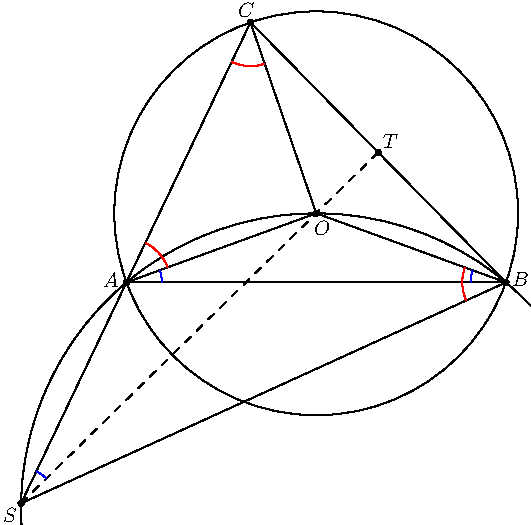
\includegraphics{g1fig.pdf}
\end{center}

\bigskip

\textbf{Marking Scheme}

\begin{itemize}
    \item 2P: Umformulierung des zu Beweisenden in eine der folgenden Aussagen:
    \begin{itemize}
    \item $\angle SCT=90^\circ-\angle CST$ oder $\angle SCB=90^\circ-\angle CSO$
    \item $CSB$ ist gleichschenklig mit Scheitelpunkt $S$
    \end{itemize}
    \item 1P: Irgendwelche nützlichen Bemerkungen bezüglich dem Sehnenviereck $AOBS$ (z.B.\ $\angle OBS=\angle CAO$ or $\angle ASO=\angle ABO$)
    \item $\leq$ 2P: 1P rgendwelche nützlichen Bemerkungen bezüglich dem Mittelpunkt $O$ des Kreises $ABC$ (z.B.\ $\angle ACO=\frac{1}{2}\cdot \angle AOB$, $\angle OCB=\angle OBC$, $\angle OCA=\angle OAC$, $\angle OBA=\angle OAB$) 
    \item 2P: Beweis vollenden
\end{itemize}
}


\fr{Soit $O$ le centre du cercle circonscrit d'un triangle aigu $ABC$. La droite $AC$ coupe le cercle circonscrit du triangle $ABO$ une deuxième fois en $S$. Montrer que la droite $OS$ est perpendiculaire à la droite $BC$.

\textbf{Solution 1:}
Reformulation de la conclusion: Pour prouver que $OS$ est perpendiculaire à $BC$, nous introduisons $T$ comme l'intersection de $OS$ avec $BC$ et montrons que $\angle CTS=90^\circ$. Par chasse aux angles, nous faisons les observations suivantes.

\begin{enumerate}
    \item Comme $AOBS$ sont sur un cercle, nous avons $\angle ASO=\angle ABO$.
    \item Comme $O$ est le centre du cercle $ABC$, on a $OA=OB$, et le triangle $AOB$ est isocèle en $O$. Ainsi $\angle AOB=180^\circ -2\cdot\angle ABO$.
    \item Comme $O$ est le centre du cercle $ABC$, on a $\angle ACB=\frac{1}{2}\cdot\angle AOB$.
\end{enumerate}

En combinant les observations ci-dessus, on obtient
\[
\angle SCT=\angle ACB\stackrel{\text{(c)}}{=}\frac{1}{2}\angle AOB\stackrel{\text{(b)}}{=}90^\circ -\angle ABO\stackrel{\text{(a)}}{=}90^\circ -\angle ASO=90^\circ -\angle CST.
\]
Ainsi, comme la somme des angles dans le triangle $CTS$ vaut $180^\circ$, on conclut :
\[
\angle CTS=180^\circ-\angle SCT-\angle CST=90^\circ.
\]

\textbf{Solution 2:}
Reformulation de la conclusion: Pour prouver que $OS$ est perpendiculaire à $BC$, on prouve que le triangle $CSB$ est isocèle en $S$. En effet, si le triangle $CSB$ était isocèle, alors la médiatrice de $BC$ contiendrait le point $S$. De plus, on peut remarquer que la médiatrice de $BC$ contient aussi $O$, puisque $OC=OB$. Ainsi, la droite $OS$ serait la médiatrice de $BC$, et serait, en particulier, perpendiculaire à $BC$. 

Par chasse aux angles, on fait les observations suivantes.

\begin{enumerate}
    \item Comme $O$ est le centre du cercle $ABC$, on a $OB=OC$ et donc $\angle OCB=\angle OBC$.
    \item Comme $O$ est le centre du cercle $ABC$, on a de façon similaire $\angle OCA=\angle OAC$.
    \item Comme $AOBS$ sont sur un cercle, nous avons que $\angle OBS=\angle OAC$.
\end{enumerate}

Ainsi, on conclut que
\[
\angle SCB=\angle ACB=\angle ACO+\angle OCB\stackrel{\text{(a)\&(b)}}{=}\angle OAC+\angle OBC\stackrel{\text{(c)}}{=}\angle OBS+\angle OBC=\angle SBC.
\]

Finalement, le triangle $CSB$ est bien isocèle en $S$.

\begin{center}
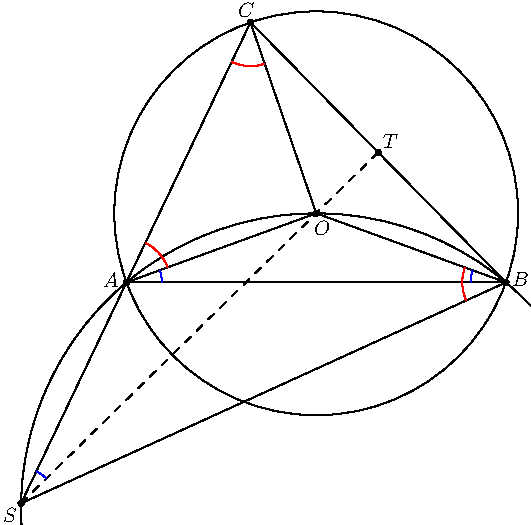
\includegraphics{g1fig.pdf}
\end{center}

\bigskip

\textbf{Marking Scheme}

\begin{itemize}
    \item 2P: Reformulation de la conclusion en une affirmation du type:
    \begin{itemize}
    \item $\angle SCT=90^\circ-\angle CST$ or $\angle SCB=90^\circ-\angle CSO$.
    \item $CSB$ est isocèle en $S$.
    \end{itemize}
    \item 1P: Toute affirmation utile utilisant le quadrilatère cyclique $AOBS$ (eg.\ $\angle OBS=\angle CAO$ ou $\angle ASO=\angle ABO$).
    \item $\leq$ 2P: 1P pour n'importe quelle affirmation utile utilisant le centre $O$ du cercle $ABC$ (eg.\ $\angle ACO=\frac{1}{2}\cdot \angle AOB$, $\angle OCB=\angle OBC$, $\angle OCA=\angle OAC$, $\angle OBA=\angle OAB$).
    \item 2P: Conclure.
\end{itemize}

}